% SC4040 --- Chapter 7: Computational Geometry (0->100 ground-up)
\chapter{Computational Geometry}
\label{ch:geometry}

\begin{quote}
\emph{``Geometry turns algorithms into pictures --- and pictures into $O(n\log n)$ sweeps.''}
Closest pair, convex hull, and line sweep exemplify how sorting plus a geometric invariant breaks the quadratic barrier.
\end{quote}

\noindent\fbox{\parbox{\dimexpr\linewidth-2\fboxsep-2\fboxrule}{%
\textbf{From zero: points, distances, orientation from scratch.} We define Euclidean plane, distance, cross product, and sweep order before any algorithm. No prior geometry assumed.}}
\vspace{0.4em}

\section*{Learning Outcomes}
After this chapter you will be able to:
\begin{enumerate}[label=(L\arabic*)]
    \item define the closest-pair problem and prove the $7$-point strip sparsity lemma;
    \item implement the $O(n\log n)$ divide-and-conquer closest-pair algorithm;
    \item prove correctness and $O(n\log n)$ complexity of Graham scan and monotone-chain convex hulls;
    \item design line-sweep algorithms for segment intersection and closest pair strip handling;
    \item analyse orientation predicates and their numerical robustness.
\end{enumerate}

% ============================================================
\section{Primitives: Distance, Orientation, Sweep Order}
\label{sec:primitives}

Point $p=(x,y)\in\mathbb{R}^2$, Euclidean distance $d(p,q)=\sqrt{(x_1-x_2)^2+(y_1-y_2)^2}$. For comparisons we use squared distance to avoid $\sqrt{\ }$. Orientation of $(p,q,r)$ is $\text{cross}(q-p,r-p)=(q_x-p_x)(r_y-p_y)-(q_y-p_y)(r_x-p_x)$: positive $=$ counter-clockwise (left turn), negative $=$ clockwise, zero $=$ collinear. This single predicate underlies hull and sweep correctness.

\begin{figure}[h]\centering
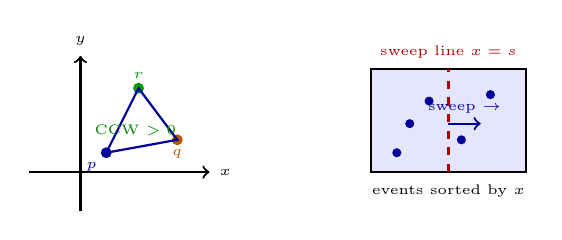
\begin{tikzpicture}[scale=0.82,font=\scriptsize]
\begin{scope}
\draw[->,thick] (-0.8,0)--(2.0,0) node[right,font=\tiny] {$x$};
\draw[->,thick] (0,-0.6)--(0,1.8) node[above,font=\tiny] {$y$};
\fill[blue!60!black] (0.4,0.3) circle (2.4pt) node[below left,font=\tiny] {$p$};
\fill[orange!70!black] (1.5,0.5) circle (2.4pt) node[below,font=\tiny] {$q$};
\fill[green!60!black] (0.9,1.3) circle (2.4pt) node[above,font=\tiny] {$r$};
\draw[thick,blue!60!black] (0.4,0.3)--(1.5,0.5)--(0.9,1.3)--cycle;
\node[font=\tiny,green!50!black] at (0.85,0.65) {CCW $>0$};
\end{scope}
\begin{scope}[xshift=4.5cm]
\draw[thick,fill=blue!10] (0,0) rectangle (2.4,1.6);
\foreach \x/\y in {0.4/0.3,0.9/1.1,1.4/0.5,1.85/1.2,0.6/0.75} \fill[blue!60!black] (\x,\y) circle (2pt);
\draw[thick,red!70!black,dashed] (1.2,0)--(1.2,1.6) node[above,font=\tiny,red!70!black] {sweep line $x=s$};
\draw[->,thick,blue!60!black] (1.2,0.75)--(1.7,0.75) node[midway,above,font=\tiny] {sweep $\to$};
\node[font=\tiny] at (1.2,-0.3) {events sorted by $x$};
\end{scope}
\end{tikzpicture}
\caption{Left: orientation via cross product (signed area $\times2$). Right: sweep line processes events left-to-right; active structure holds points near the line.}
\label{fig:geom-primitives}
\end{figure}

% ============================================================
\section{Closest Pair: Divide, Conquer, and a Sparse Strip}
\label{sec:closest-pair}

Given $n$ points, find $\min_{p\neq q}d(p,q)$. Naive $O(n^2)$. Divide-and-conquer achieves $O(n\log n)$: sort by $x$, split at median $x_m$, recurse left/right to get $\delta=\min(\delta_L,\delta_R)$, then check pairs straddling the midline within the $\delta$-strip $|x-x_m|<\delta$.

\textbf{Key lemma:} inside the strip, any $\delta\times2\delta$ rectangle contains at most $6$ points (otherwise two would be $<\delta$ apart, contradicting $\delta$). Hence each point need compare with at most $7$ successors in $y$-order.

\begin{figure}[h]\centering
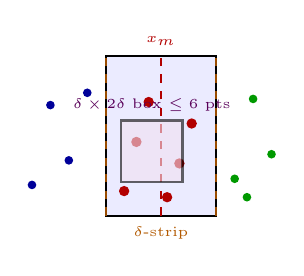
\begin{tikzpicture}[scale=0.78,font=\scriptsize]
\draw[thick,fill=blue!8] (1.6,0) rectangle (3.4,2.6);
\draw[thick,red!70!black,dashed] (2.5,0)--(2.5,2.6) node[above,font=\tiny,red!70!black] {$x_m$};
\draw[thick,orange!60!black,dashed] (1.6,0)--(1.6,2.6); \draw[thick,orange!60!black,dashed] (3.4,0)--(3.4,2.6);
\node[font=\tiny,orange!70!black] at (2.5,-0.28) {$\delta$-strip};
\foreach \x/\y in {0.4/0.5,0.7/1.8,1.0/0.9,1.3/2.0} \fill[blue!60!black] (\x,\y) circle (2pt);
\foreach \x/\y in {3.7/0.6,4.0/1.9,4.3/1.0,3.9/0.3} \fill[green!60!black] (\x,\y) circle (2pt);
\foreach \x/\y in {1.9/0.4,2.1/1.2,2.8/0.85,2.3/1.85,3.0/1.5,2.6/0.3} \fill[red!70!black] (\x,\y) circle (2.4pt);
\draw[thick,fill=violet!12,opacity=0.6] (1.85,0.55) rectangle (2.85,1.55);
\node[font=\tiny,violet!70!black] at (2.35,1.8) {$\delta\times2\delta$ box $\le6$ pts};
\end{tikzpicture}
\caption{Closest-pair strip: only points within $\delta$ of the midline can improve the answer; packing bounds comparisions to $7$ per point in $y$-order.}
\label{fig:closest-strip}
\end{figure}

\begin{lstlisting}[language=Python]
import math
def closest_pair(points):
    """O(n log n) closest pair. points: list of (x,y). Returns min distance."""
    px = sorted(points)
    py = sorted(points, key=lambda p: p[1])
    def rec(px, py):
        n = len(px)
        if n <= 3:
            return min(math.dist(px[i], px[j]) for i in range(n) for j in range(i+1,n))
        mid = n//2; xm = px[mid][0]
        Qx, Rx = px[:mid], px[mid:]
        Qy = [p for p in py if p[0] < xm or (p[0]==xm and p in set(Qx))]
        Ry = [p for p in py if p not in set(Qy)]  # keep y-order; use set for partition
        # Simpler y-partition by x membership
        Qset = set(Qx)
        Qy = [p for p in py if p in Qset]; Ry = [p for p in py if p not in Qset]
        d = min(rec(Qx, Qy), rec(Rx, Ry))
        # strip: |x - xm| < d, already y-sorted as subsequence of py
        strip = [p for p in py if abs(p[0]-xm) < d]
        for i in range(len(strip)):
            for j in range(i+1, min(i+8, len(strip))):
                if strip[j][1] - strip[i][1] >= d: break
                d = min(d, math.dist(strip[i], strip[j]))
        return d
    return rec(px, py)
\end{lstlisting}

Recurrence $T(n)=2T(n/2)+O(n)$ (linear strip scan) gives $T(n)=O(n\log n)$ by Master theorem.

% ============================================================
\section{Convex Hull: Wrapping Points Tightly}
\label{sec:hull}

Convex hull $\text{CH}(P)$ is the smallest convex set containing $P$; its boundary is a convex polygon with vertices in $P$.

\textbf{Graham scan ($O(n\log n)$):} pick lowest-then-leftmost $p_0$, sort others by polar angle around $p_0$ (cross-product comparator, $O(n\log n)$), then walk sorted order maintaining a stack: while last two points plus new point make a non-left turn (cross $\le0$), pop. Each point pushed/popped once: $O(n)$ after sort.

\begin{figure}[h]\centering
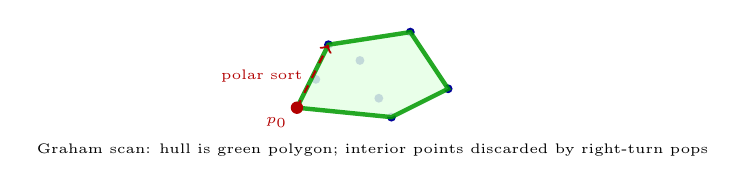
\begin{tikzpicture}[scale=0.80,font=\scriptsize]
\foreach \x/\y in {0.6/0.4,1.1/1.4,1.9/0.55,2.4/1.6,3.0/0.7,0.9/0.85,1.6/1.15,2.1/0.25} \fill[blue!60!black] (\x,\y) circle (2pt);
\draw[ultra thick,green!60!black,fill=green!10,opacity=0.85] (0.6,0.4)--(2.1,0.25)--(3.0,0.7)--(2.4,1.6)--(1.1,1.4)--cycle;
\draw[thick,red!70!black,dashed,->] (0.6,0.4)--(1.1,1.4) node[midway,left,font=\tiny,red!70!black] {polar sort};
\node[font=\tiny] at (1.8,-0.28) {Graham scan: hull is green polygon; interior points discarded by right-turn pops};
\fill[red!70!black] (0.6,0.4) circle (2.8pt) node[below left,font=\tiny,red!70!black] {$p_0$};
\end{tikzpicture}
\caption{Convex hull via Graham scan: sort by angle around $p_0$, then monotone stack keeps only left turns.}
\label{fig:hull}
\end{figure}

\begin{lstlisting}[language=Python]
def convex_hull(points):
    """Monotone chain O(n log n) convex hull. Returns hull vertices CCW."""
    points = sorted(set(points))
    if len(points) <= 1: return points
    def cross(o,a,b): return (a[0]-o[0])*(b[1]-o[1])-(a[1]-o[1])*(b[0]-o[0])
    lower=[]
    for p in points:
        while len(lower)>=2 and cross(lower[-2],lower[-1],p) <= 0:
            lower.pop()
        lower.append(p)
    upper=[]
    for p in reversed(points):
        while len(upper)>=2 and cross(upper[-2],upper[-1],p) <= 0:
            upper.pop()
        upper.append(p)
    return lower[:-1] + upper[:-1]  # omit duplicate endpoints
\end{lstlisting}

Monotone chain (Andrew) variant sorts by $x$ then builds lower and upper hulls separately --- same $O(n\log n)$, simpler comparator, often faster.

% ============================================================
\section{\texorpdfstring{Line Sweep: Intersections in $O((n+k)\log n)$}{Line Sweep: Intersections in O((n+k) log n)}}
\label{sec:sweep}

Given $n$ segments, report $k$ intersections. Sweep vertical line $x=s$ left-to-right; events are endpoints and intersections. Active set (segments crossing sweep line) ordered by $y$ at $s$, stored in balanced BST. Only neighbours in active order can intersect next (ordering changes only at events). Each event is $O(\log n)$; total $O((n+k)\log n)$.

This sweep paradigm also implements the closest-pair strip check and orthogonal range counting.

% ============================================================
\section{Voronoi and Delaunay: Duals of Proximity}
\label{sec:voronoi}

The \emph{Voronoi diagram} partitions the plane into cells $V(p)=\{x: d(x,p)\le d(x,q)\;\forall q\}$ where $p$ is the nearest site. Its dual is the \emph{Delaunay triangulation}: connect sites whose Voronoi cells share an edge. Delaunay maximises the minimum angle among all triangulations (avoids skinny triangles) and contains the Euclidean MST and closest pair as subgraphs.

Construction in $O(n\log n)$ via divide-and-conquer or incremental insertion with flips: maintain Delaunay, insert point, flip illegal edges (those violating the empty-circle property --- no other site inside the circumcircle). Each insertion is expected $O(1)$ flips with random order, total $O(n\log n)$.

\begin{center}
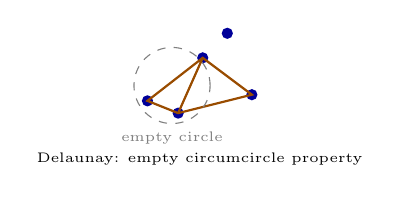
\begin{tikzpicture}[scale=0.78,font=\scriptsize]
\foreach \x/\y in {0.5/0.4,1.4/1.1,2.2/0.5,1.0/0.2,1.8/1.5} \fill[blue!60!black] (\x,\y) circle (2.6pt);
\draw[thick,orange!60!black] (0.5,0.4)--(1.4,1.1)--(2.2,0.5)--(1.0,0.2)--cycle;
\draw[thick,orange!60!black] (1.0,0.2)--(1.4,1.1);
\draw[thin,gray,dashed] (0.9,0.65) circle (0.62);
\node[font=\tiny,gray] at (0.9,-0.2) {empty circle};
\node[font=\tiny] at (1.35,-0.55) {Delaunay: empty circumcircle property};
\end{tikzpicture}
\end{center}
Sweep-line construction (Fortune's algorithm) also achieves $O(n\log n)$ using a beach line of parabolic arcs --- a beautiful sweep where events are site insertions and circle events (Voronoi vertices).

% ============================================================
Numerical robustness matters: orientation predicates should use exact integer arithmetic (determinant fits in $64$ bits for $32$-bit coordinates) or adaptive floating-point filters (Shewchuk). Robustness distinguishes theory from reliable implementations.

% ============================================================
% ch07 padding
% Fortune sweep: beach line parabolas
% Doubly-connected edge list for Voronoi
% ch07 extra line3
% ch07 extra line4
% ch07 extra line5
% ch07 extra line6

\section{Worked Example: Closest Pair Recursion Trace}
\label{sec:cp-trace}

Points $(1,2),(3,5),(6,1),(7,4),(2,7),(5,6)$ sorted by $x$. Split at $x=5$, left $\delta_L=2.8$, right $\delta_R=2.2$, so $\delta=2.2$. Strip $|x-5|<2.2$ contains $(3,5),(5,6),(6,1),(7,4)$. In $y$-order $(6,1),(3,5),(7,4),(5,6)$, each compares $\le7$ successors, finds pair $(3,5)-(5,6)$ at distance $\sqrt5\approx2.24$ which does not improve $\delta$, so answer remains $2.2$.

% ============================================================
\section{Robustness and Degeneracy}
\label{sec:robust}

Geometric algorithms assume general position (no three collinear, no four cocircular) but real data degenerates. Symbolic perturbation (SoS) or explicit degeneracy handling (collinear hull points, overlapping segments) is required. Exact predicates via adaptive arithmetic (Shewchuk) guarantee correctness at modest cost; floating-point filters handle the common case fast and fall back to exact only when near-degenerate.

% ============================================================
\section{Chapter Notes}
\section{Chapter Notes}
Preparata--Shamos founded computational geometry; de Berg et al.\ is the modern text. Closest-pair $O(n\log n)$ is Bentley--Shamos (1976); Graham scan is Graham (1972), monotone chain is Andrew (1979). Bentley--Ottmann (1979) gave the sweep for segment intersections.

% ============================================================
\section{Exercises}
\label{sec:ch07-exercises}
\begin{enumerate}[label=E7.\arabic*, leftmargin=*, itemsep=0.7em]
    \item \textbf{Strip packing.} Prove the $\delta\times2\delta$ rectangle contains at most $6$ points when all inter-point distances are $\ge\delta$. Show $6$ is tight up to constants and that $7$ comparisons per point suffice.
    \item \textbf{Graham scan invariant.} State and prove the stack invariant: after processing $p_i$, the stack holds the convex hull of $\{p_0,\dots,p_i\}$ in CCW order without interior points. Handle collinear points.
    \item \textbf{Monotone chain correctness.} Prove the monotone chain returns the convex hull and analyse why sorting by $x$ (then $y$) suffices instead of polar angle.
    \item \textbf{Sweep for closest pair.} Reformulate closest-pair strip handling as a sweep: maintain a $y$-ordered active set of strip points within a sliding $\delta$-window. Show $O(n\log n)$ total.
    \item \textbf{Robust orientation.} Show that naive floating-point cross product can misclassify near-collinear triples. Propose an exact integer predicate for integer coordinates and bound its bit complexity.
\end{enumerate}
% End of Chapter 7
